%Beamer class
\documentclass{beamer}

\usepackage[czech]{babel}
\usepackage[utf8]{inputenc}
\usepackage{fontenc}
\usepackage{tgheros}
\usepackage{array}
\usepackage{color}
\usepackage{hyperref}
\usepackage{fancyvrb} % pro verbatim

\usetheme{AnnArbor}
\usecolortheme{crane}


\title[KiCAD Eeschema]{Tvorba schéma zapojení v KiCAD}
\subtitle[KEO] {Konstrukce a realizace elektronických obvodů}
\author[Brejcha]{\texorpdfstring{Michal Brejcha\newline\url{brejcmic@fel.cvut.cz}}{Michal Brejcha}}
\institute[ČVUT]{ČVUT v Praze, FEL}
\date[Praha, 2021]{Praha, 2021}

%------------------------------------------------------------------------------
%Konstanty a definice
%------------------------------------------------------------------------------
\newtheorem{myDef}{}
\newcommand{\kicadVersion}{5.1.10.}

\begin{document}
%------------------------------------------------------------------------------
%Uvodni slajd
%------------------------------------------------------------------------------
\frame{\titlepage}

\begin{frame}
\frametitle{Obsah} 
\tableofcontents
\end{frame}

\AtBeginSection[]
{
  \begin{frame}
    \frametitle{Téma}
    \tableofcontents[currentsection]
  \end{frame}
}

%------------------------------------------------------------------------------
% Založení projektu
%------------------------------------------------------------------------------
\section{\texorpdfstring{Založení projektu}{Zalozeni projektu}}
\subsection{\texorpdfstring{Příprava nového projektu}{Priprava noveho projektu}}
%------------------------------------------------------------------------------
\begin{frame}
	\frametitle{Nový projekt}
	\begin{columns}
	
		\column{.5\textwidth}
		\begin{center}
			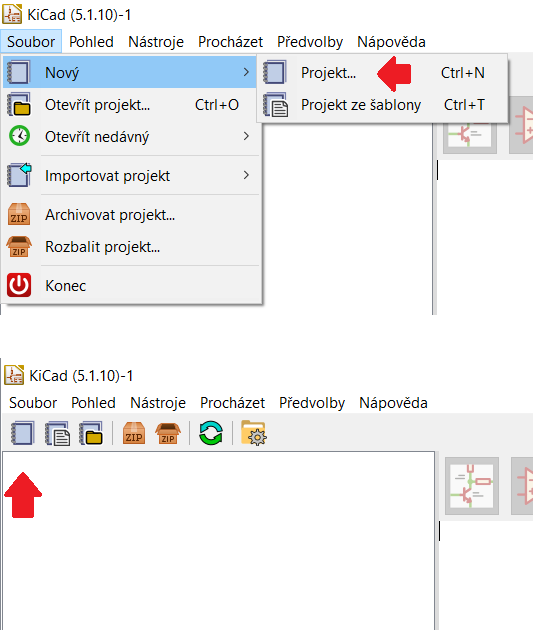
\includegraphics[width=\textwidth]{obr/prj_novy01.png}
		\end{center}
	
		\column{.5\textwidth}
		\textbf{Možnosti:}
		\begin{itemize}
			\item $\downarrow$ Soubor $\downarrow$ Nový $\downarrow$ Projekt
			\item CTRL+N
			\item Modrá ikona notýsku úplně vlevo
		\end{itemize}
	\end{columns}
\end{frame}
%------------------------------------------------------------------------------
\begin{frame}
	\frametitle{Nový projekt}

		\begin{center}
			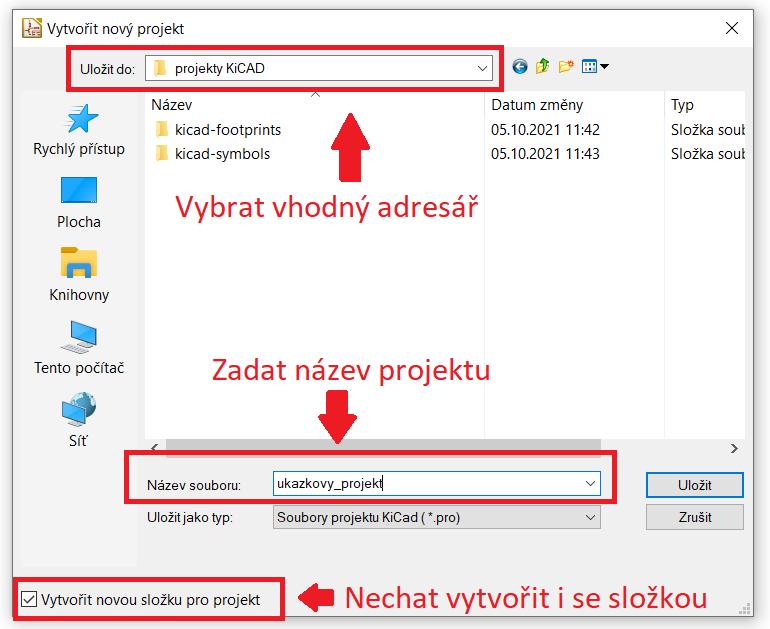
\includegraphics[width=0.7\textwidth]{obr/prj_novy02.png}
		\end{center}
    
\end{frame}
%------------------------------------------------------------------------------
\begin{frame}
	\frametitle{Aktivní projekt}

		\begin{center}
			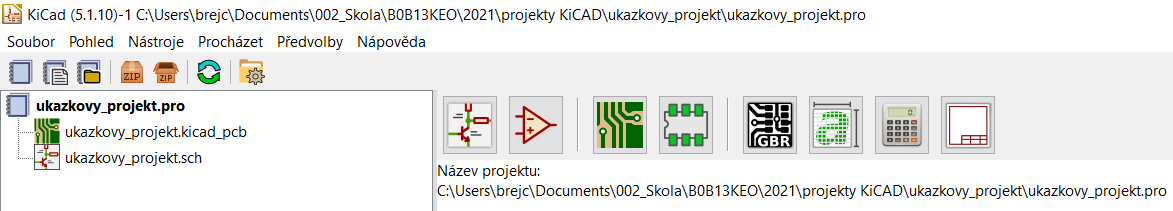
\includegraphics[width=\textwidth]{obr/prj_novy03.png}
		\end{center}
    
		
		\begin{itemize}
			\item Vlevo se je souborová struktura projektu,
			\item ikony pro jednotlivé programy (Návrh schématu, Editor součástek, atd.) jsou aktivní a programy automaticky pracují s projektovými soubory.
		\end{itemize}
		
\end{frame}
%------------------------------------------------------------------------------


%------------------------------------------------------------------------------
\subsection{\texorpdfstring{Přidání vlastních knihoven}{Pridani vlastnich knihoven}}
%------------------------------------------------------------------------------
\begin{frame}
	\frametitle{Zadání cest k vlastním knihovnám}
	\begin{columns}
	
		\small
		\column{.45\textwidth}
		\textbf{Dva typy knihoven:}
		\begin{itemize}
			\item schématické značky a
			\item pouzdra.
		\end{itemize}
		
		\textbf{Editace cest:}
		\begin{enumerate}
			\item přímo z projektového menu,
			\item pro schématické značky z programu \uv{Editor schémat},
			\item pro pouzdra z programu \uv{Návrh DPS},
		\end{enumerate}
		
		\textbf{Vždy pomocí:}
		
		$\downarrow$ Předvolby $\downarrow$ Správa knihoven $[$součástek $|$ pouzder$]$
	
		\column{.55\textwidth}
		\begin{center}
			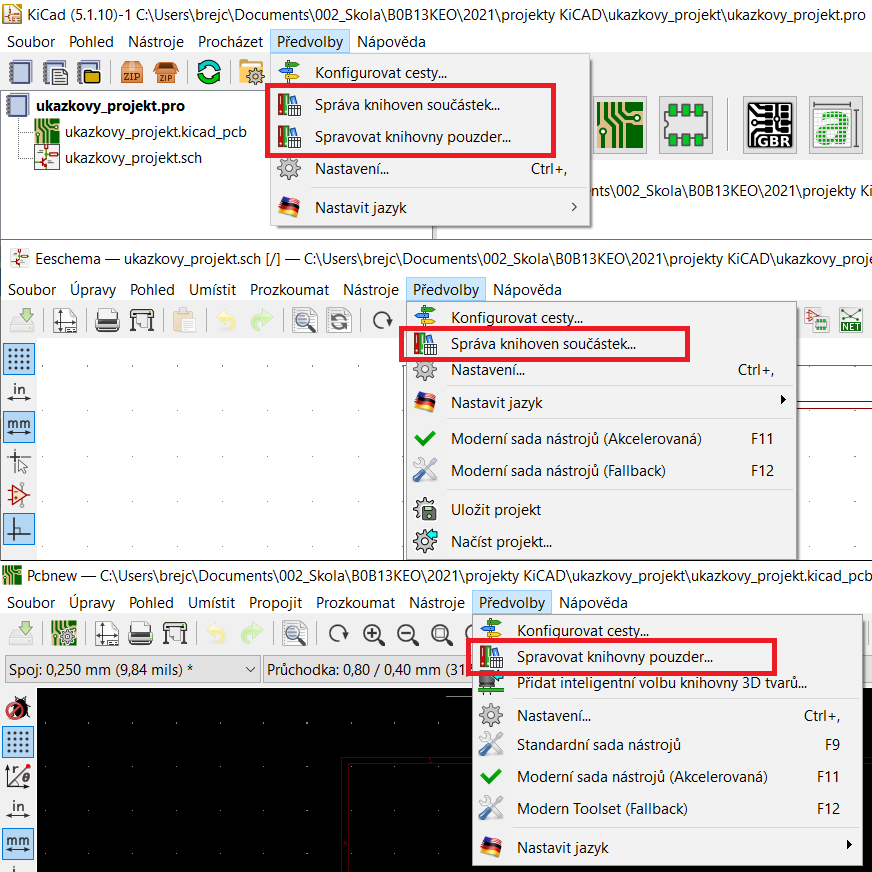
\includegraphics[width=\textwidth]{obr/knihovny01.png}
		\end{center}
	
	\end{columns}
\end{frame}
%------------------------------------------------------------------------------
\begin{frame}
	\frametitle{Zadání cest k vlastním knihovnám}
	
	\textbf{Cesty ke knihovnám jsou:}
	\begin{itemize}
		\item \uv{Globální}, pak platí pro jakýkoliv projekt na daném PC,
		\item \uv{Specifické pro projekt}, pak se týkají jen konkrétního projektu.
	\end{itemize}
	
	\vspace{0.3cm}
	V rámci předmětu B0B13KEO nebudeme nahrazovat cesty ke globálním knihovnám. Pouze je deaktivujeme a jako aktivní označíme přidané projektové knihovny.
	
	\vspace{0.3cm}
	Cesty ke knihovnám se ukládají a dají měnit editováním textových souborů:
	
	\begin{itemize}
		\item sym-lib-table
		\item fp-lib-table
	\end{itemize}
		
\end{frame}
%------------------------------------------------------------------------------
\begin{frame}
	\frametitle{Zadání cest ke knihovnám - schematické značky}

		\begin{center}
			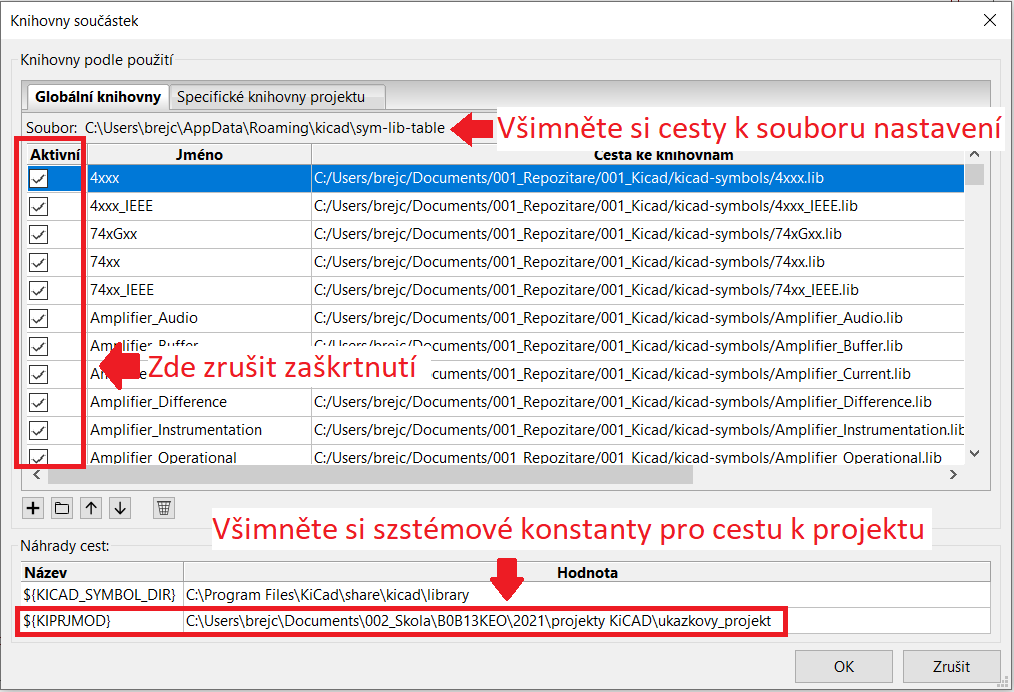
\includegraphics[width=0.85\textwidth]{obr/knihovny02.png}
		\end{center}
		
\end{frame}
%------------------------------------------------------------------------------
\begin{frame}
	\frametitle{Zadání cest ke knihovnám - schematické značky}

		\begin{center}
			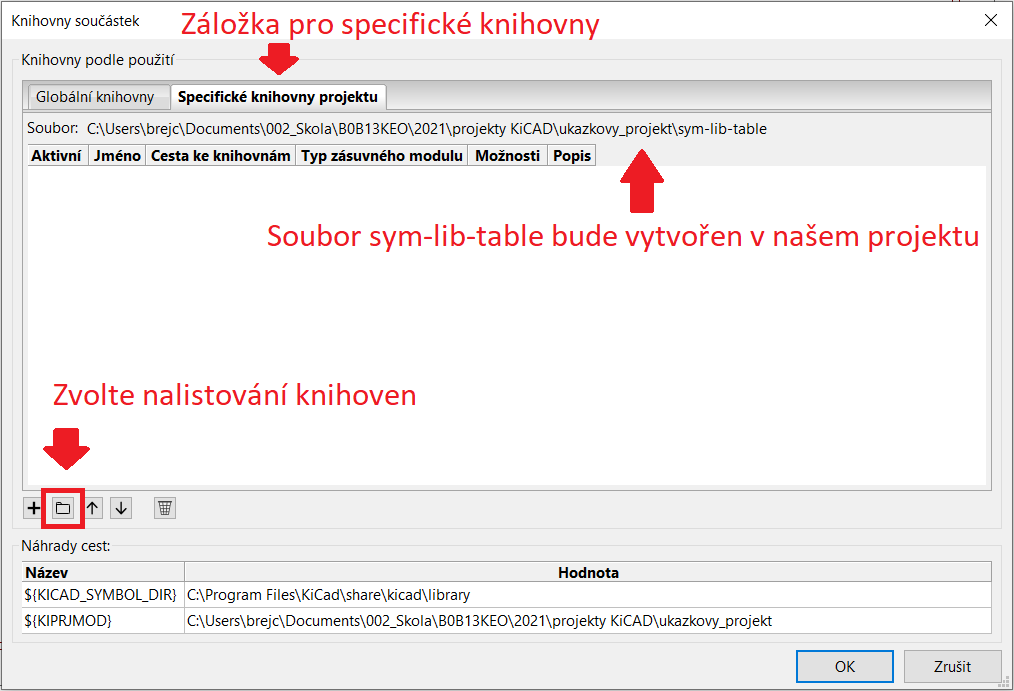
\includegraphics[width=0.85\textwidth]{obr/knihovny03.png}
		\end{center}
		
\end{frame}
%------------------------------------------------------------------------------
\begin{frame}
	\frametitle{Zadání cest ke knihovnám - schematické značky}

		\begin{center}
			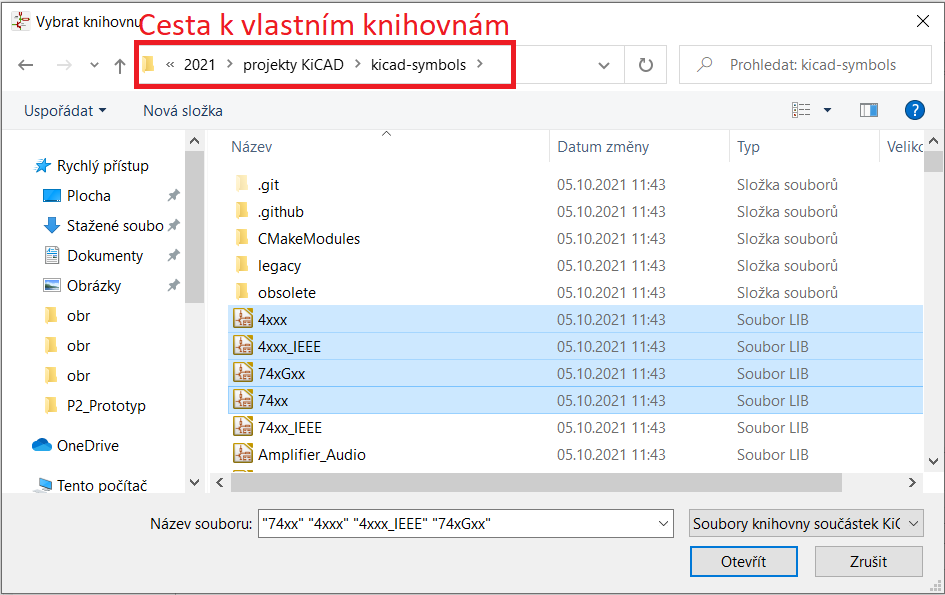
\includegraphics[width=0.7\textwidth]{obr/knihovny04.png}
		\end{center}
	  
		\begin{itemize}
			\item Nastavte cetu k vlastním knohovnám
			\item a pomocí klávesy shift nebo ctrl vyberte všechny soubory *.lib
		\end{itemize}
\end{frame}
%------------------------------------------------------------------------------
\begin{frame}
	\frametitle{Zadání cest ke knihovnám - schematické značky}

		\begin{center}
			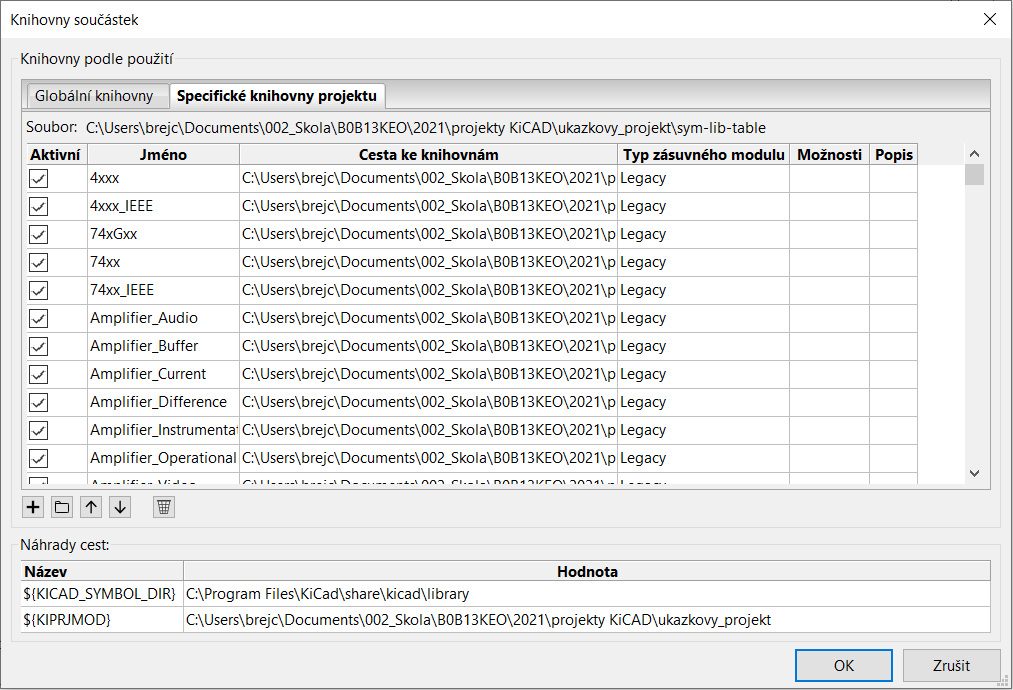
\includegraphics[width=0.85\textwidth]{obr/knihovny05.png}
		\end{center}
		
\end{frame}
%------------------------------------------------------------------------------
\begin{frame}[fragile]
	\frametitle{Zadání cest k vlastním knihovnám}
	\small
	Všimněte si, že všechny soubory jsou zadány absolutní cestou. To může být nevýhodné, pokud s někým sdílíte projekt nebo zálohujete tento projekt na jiném počítači (GIT apod.).
	
	\vspace{3mm}
	Nejvhodnější způsob je zadání relativních cest pomocí systémové proměnné \$$\{$KIPRJMOD$\}$, která ukazuje na adresář našeho projektu.
	
	\vspace{3mm}
	Jelikož vkládané knihovny jsou v našem případě ve stejné složce jako projekty, je nutné přepsat začátek všech cest:
	
	\begin{verbatim*}
		C:\Users\brejc\Documents\002_Skola\B0B13KEO\2021\projekty_KiCAD\
	\end{verbatim*}
	
	na tvar:
	
	\$\verb+{KIPRJMOD}/../+
		
\end{frame}
%------------------------------------------------------------------------------
\begin{frame}
	\frametitle{Zadání cest ke knihovnám - schematické značky}

		\begin{center}
			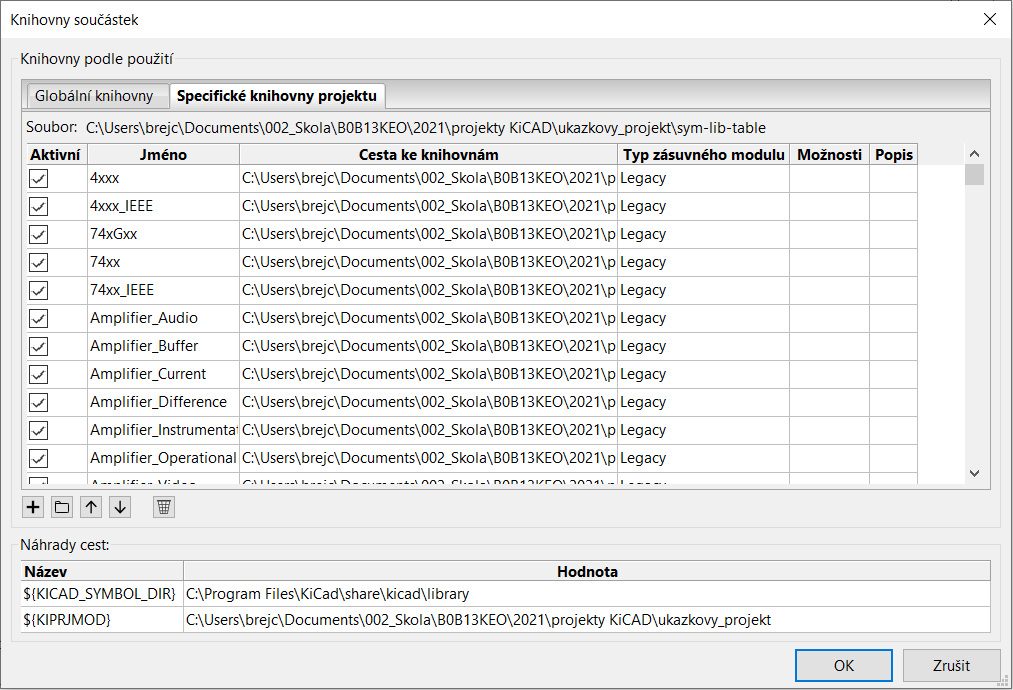
\includegraphics[width=0.85\textwidth]{obr/knihovny05.png}
		\end{center}
		
\end{frame}
%------------------------------------------------------------------------------
\begin{frame}
	\frametitle{Zadání cest ke knihovnám - schematické značky}

		\begin{center}
			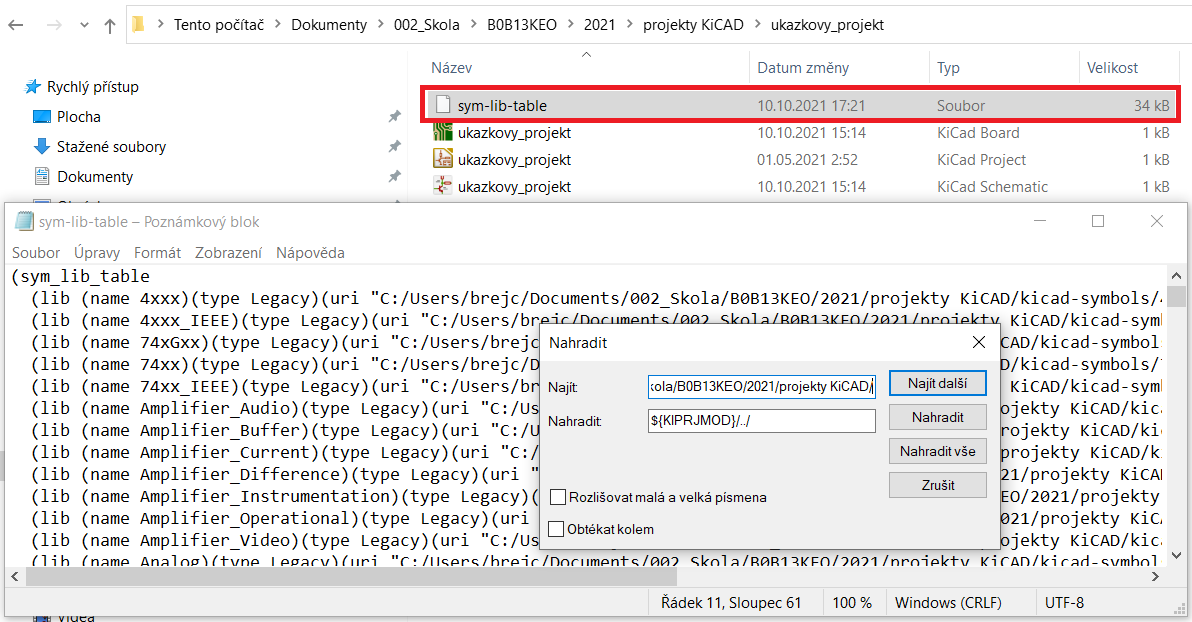
\includegraphics[width=0.85\textwidth]{obr/knihovny06.png}
		\end{center}
		
		Praktickou cestou je otevření projektového souboru sym-lib-table v poznámkovém bloku a provedení hromadného nahrazení textu.
\end{frame}
%------------------------------------------------------------------------------
\begin{frame}
	\frametitle{Zadání cest ke knihovnám - schematické značky}

		\begin{center}
			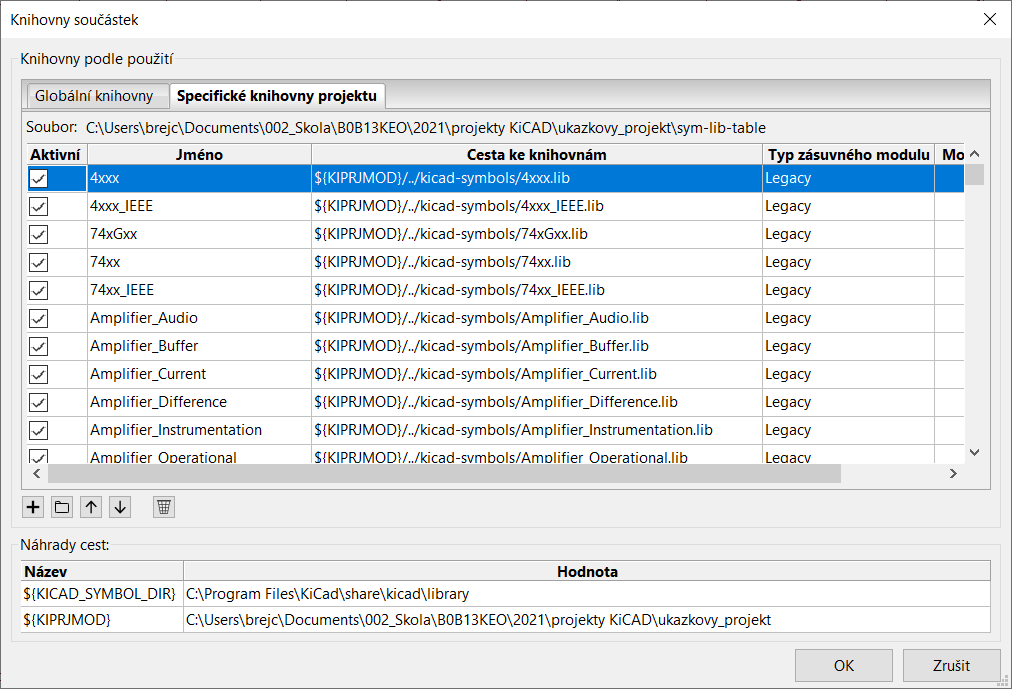
\includegraphics[width=0.85\textwidth]{obr/knihovny07.png}
		\end{center}
		
\end{frame}
%------------------------------------------------------------------------------
\begin{frame}
	\frametitle{Zadání cest ke knihovnám - pouzdra}
		
		Téměř identický postup je třeba udělat ještě pro knihovny pouzder. Zde zadáváme cesty k adresářům s koncovkou *.pretty
		
		\vspace{3mm}
		Při zadávání dejte pozor, ať \textbf{nepřidáváte tyto adresáře}:
		
		\begin{itemize}
		  \item .github
			\item CMakeModules,
		  \item Obsolete,
			\item Sources.
		\end{itemize}
		
		Tyto adresáře jsou vždy součástí stažených knihoven a nejedná se o knihovní prvky.
		
		\vspace{3mm}
		Změnu absolutních cest na relativní proveďte ve vytvořeném souboru fp-lib-table.
\end{frame}
%------------------------------------------------------------------------------
\begin{frame}
	\frametitle{Zadání cest ke knihovnám - pouzdra}

		\begin{center}
			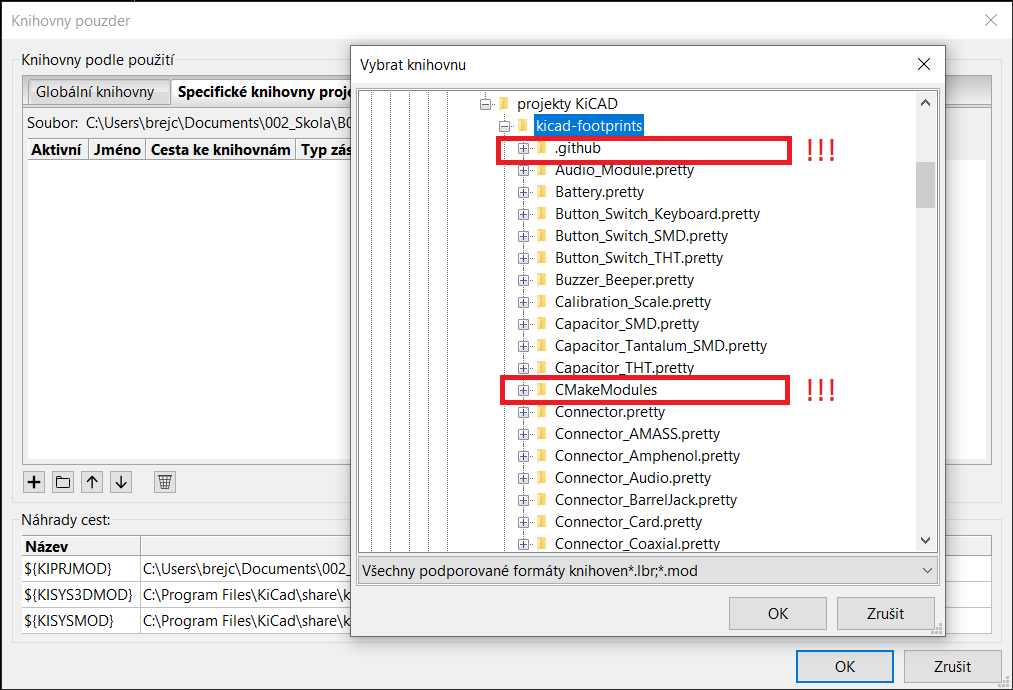
\includegraphics[width=0.85\textwidth]{obr/knihovny08.png}
		\end{center}
		
\end{frame}
%------------------------------------------------------------------------------

%------------------------------------------------------------------------------
% Eeschema
%------------------------------------------------------------------------------
\section{\texorpdfstring{Schéma zapojení}{Schema zapojeni}}
\subsection{\texorpdfstring{Volba stránky a razítko}{Volba stranky a razitko}}
%------------------------------------------------------------------------------
\begin{frame}
	\frametitle{Volba stránky a razítko}
		
\end{frame}
%------------------------------------------------------------------------------


%------------------------------------------------------------------------------
\subsection{\texorpdfstring{Vkládání součástek}{Vkladani soucastek}}
%------------------------------------------------------------------------------
\begin{frame}
	\frametitle{Výběr a vložení součástky}
		
\end{frame}
%------------------------------------------------------------------------------


%------------------------------------------------------------------------------
\subsection{\texorpdfstring{Propojování - vodiče a odkazy}{Propojovani - vodice a odkazy}}
%------------------------------------------------------------------------------
\begin{frame}
	\frametitle{Propojování součástek}
		
\end{frame}
%------------------------------------------------------------------------------


%------------------------------------------------------------------------------
\subsection{\texorpdfstring{Tvorba nových listů}{Tvorba novych listu}}
%------------------------------------------------------------------------------
\begin{frame}
	\frametitle{Přidávání stránek}
		
\end{frame}
%------------------------------------------------------------------------------


%------------------------------------------------------------------------------
\subsection{\texorpdfstring{Kontrola zapojení}{Kontrola zapojeni}}
%------------------------------------------------------------------------------
\begin{frame}
	\frametitle{Kontrola zapojení}
		
\end{frame}
%------------------------------------------------------------------------------


%------------------------------------------------------------------------------
\subsection{\texorpdfstring{Přiřazení pouzder}{Prirazeni pouzder}}
%------------------------------------------------------------------------------
\begin{frame}
	\frametitle{Přiřazování pouzder}
		
\end{frame}
%------------------------------------------------------------------------------

  
\end{document}